
% --------------------------------------------------------------
% This is all preamble stuff that you don't have to worry about.
% Head down to where it says "Start here"
% --------------------------------------------------------------
 
\documentclass[12pt]{article}
 
\usepackage[nouppercase,headsepline,footsepline,plainfootsepline]{scrpage2}
\automark{section}
\pagestyle{scrheadings}
%\clearscrheadfoot
\ihead{Midterm2 Practice Questions}
%\ofoot[\pagemark]{\pagemark}% Optional argument controls chapter-starting pages
\ifoot[(Author)]{{\sl \hfill Meenmo K.}}

\usepackage[margin=1in]{geometry} 
\usepackage{amsmath,amsthm,amssymb,scrextend}
\usepackage{fancyhdr}
\usepackage{enumitem}
\usepackage{amsmath}
\usepackage{amssymb}
\usepackage{textcomp}
\usepackage{fancybox}
\usepackage{tikz}
\usepackage{cancel}
\usepackage{tasks}


\newcommand{\N}{\mathbb{N}}
\newcommand{\Z}{\mathbb{Z}}
\newcommand{\I}{\mathbb{I}}
\newcommand{\R}{\mathbb{R}}
\newcommand{\Q}{\mathbb{Q}}
\renewcommand{\qed}{\hfill$\blacksquare$}
\let\newproof\proof
\renewenvironment{proof}{\begin{addmargin}[1em]{0em}\begin{newproof}}{\end{newproof}\end{addmargin}\qed}
% \newcommand{\expl}[1]{\text{\hfill[#1]}$}
\setlength{\parindent}{0pt}
\newenvironment{theorem}[2][Theorem]{\begin{trivlist}
\item[\hskip \labelsep {\bfseries #1}\hskip \labelsep {\bfseries #2.}]}{\end{trivlist}}
\newenvironment{lemma}[2][Lemma]{\begin{trivlist}
\item[\hskip \labelsep {\bfseries #1}\hskip \labelsep {\bfseries #2.}]}{\end{trivlist}}
\newenvironment{problem}[2][Problem]{\begin{trivlist}
\item[\hskip \labelsep {\bfseries #1}\hskip \labelsep {\bfseries #2.}]}{\end{trivlist}}
\newenvironment{exercise}[2][Exercise]{\begin{trivlist}
\item[\hskip \labelsep {\bfseries #1}\hskip \labelsep {\bfseries #2.}]}{\end{trivlist}}
\newenvironment{reflection}[2][Reflection]{\begin{trivlist}
\item[\hskip \labelsep {\bfseries #1}\hskip \labelsep {\bfseries #2.}]}{\end{trivlist}}
\newenvironment{proposition}[2][Proposition]{\begin{trivlist}
\item[\hskip \labelsep {\bfseries #1}\hskip \labelsep {\bfseries #2.}]}{\end{trivlist}}
\newenvironment{corollary}[2][Corollary]{\begin{trivlist}
\item[\hskip \labelsep {\bfseries #1}\hskip \labelsep {\bfseries #2.}]}{\end{trivlist}}
 
 
\begin{document}
{\bf Question 1}
\begin{enumerate}[label=(\roman*)]
    \item Let $(X, d)$ be a metric space. Give the definition of $x_n\to x$ in X.\\
    
    A sequence converges if 
    $$\forall\; \epsilon>0\;\; \exists\;N>\mathbb{N} \text{ such that } d(x_n,x) \text{ if $n\ge N $}    $$
    
    \item Show that a sequence in a metric space can have at most one limit.\\
    
    Let $(X,d)$ be a metric space and $(x_n)$ be a sequence in $X$ such that
    $$x_n\to p\in X,\; x_n\to q\in X$$
    
    Since $(x_n)$ converges to $p,q$ respectively
    $$\forall\;\epsilon>0\;\;\exists\;N_1\in\mathbb{N} \text{ such that } d(x_n,p)<\frac{\epsilon}{2} \text{ if } n\ge N_1 $$
    $$\forall\;\epsilon>0\;\;\exists\;N_2\in\mathbb{N} \text{ such that } d(x_n,q)<\frac{\epsilon}{2} \text{ if } m\ge N_2 $$
    
    Let $N=\max\{N_1,N_2\}$. Then for all $m,n\ge N$
    $$d(p,q) \le d(p,x_n)+d(x_n,q) < \frac{\epsilon}{2}+\frac{\epsilon}{2} < \epsilon  $$
    Since $\epsilon$ is arbitrary, $d(p,q)=0$. Hence we proved $p=q$, implying there exists a distinct limit point in a metric space.
    
    \item Define a Cauchy sequence in a metric space.\\
    
    A sequence is Cauchy if 
    $$\forall\;\epsilon>0\;\;\exists\;N\in\mathbb{N}\text{ such that } d(x_n,x_m)<\epsilon \text{ if $n,m\ge N$} $$
    
    \item Show that every convergent sequence is Cauchy.\\
    
    Suppose $(x_n)$ is convergent to $x$. Then
    $$\forall\;\epsilon>0\;\;\exists\;N\in\mathbb{N} \text{ such that } d(x_n,x)<\frac{\epsilon}{2} \text{ if } n\ge N $$
    If $m,n \le N$, then
    $$|x_n-x_m| \le |x_n-x+x-x_m| \le |x_n-x|+|x-x_m| < \frac{\epsilon}{2}+\frac{\epsilon}{2}<\epsilon    $$
    \item Define "complete metric space".\\
    Metric space is a space where every Cauchy sequence converges
    
    \item Is every complete metric space compact?\\
    No. In case of $\mathbb{R}$, every convergent sequence in $\mathbb{R}$ converges, but $\mathbb{R}$ is unable to be covered by finite sub-covers.
    
    \item Is every compact metric space complete?
    \begin{itemize}
        \item Suppose $(x_n)\in K \subset X$ where $(x_n)$ is a Cauchy sequence, $K$ is a compact set, and $X$ is a metric space.
        \item By the theorem, we know that $(x_n)$ in the compact set $K$ has a convergent subsequent. 
        \item And as a subsequence of a Cauchy converges, every $(x_n)$ has a convergent subsequence. 
        \item This implies that every term of $(x_n)$ converges.
        \item Hence $K$ is complete.
    \end{itemize}
    
    
    \item Show that every closed subset of a compact set is compact.
    \begin{itemize}
        \item Suppose $F\subset K\subset X$ where $F$ is a closed set and $K$ is a compact set.
        \item Let $\{V_\alpha\}$ be an open cover of $F$ and $\{U_\alpha\}$ be an open cover of $K$.
        \item Since $K$ is compact, $\exists$ a finite subcovers that also covers $F$.
        \item Hence we conclude that there exists a finite sub-collection of $\{U_\alpha\}$ that covers $F$. 
        \item This gives that $F$ is a compact set also.
    \end{itemize}
    $$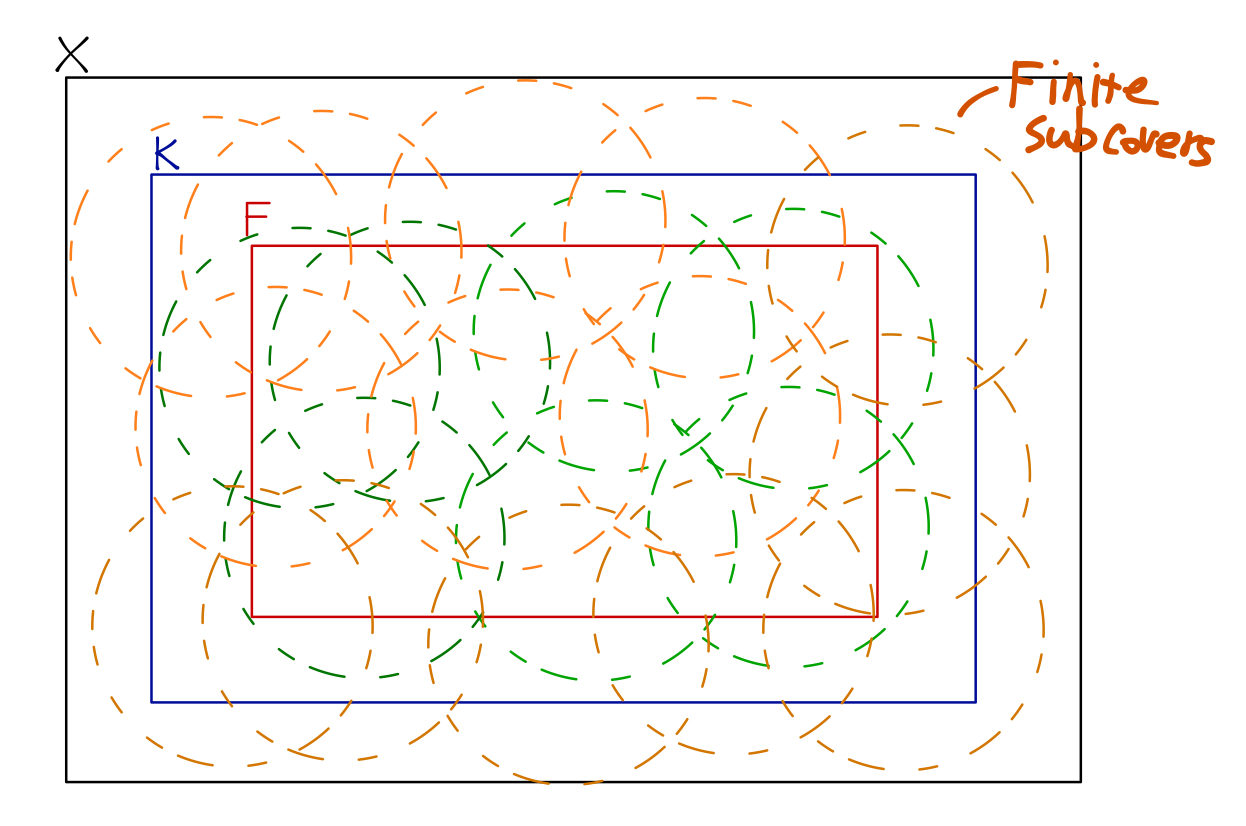
\includegraphics[height=6cm, width=13cm]{compact.jpeg}$$
    
\end{enumerate}


\end{document}